% Part I -- Linear theory
% Included from large-wave-effect.tex; preamble macros (\LN, \Q, \eu, ...),
% \graphicspath and the bibliography all live in the root file.

\section{Toeplitz and circulant matrices: a unified language}\label{sec:setting}

The bead chain is a spring--mass lattice whose stiffness operator is shift invariant---hence
Toeplitz---and, under periodic boundary conditions, circulant (Figure~\ref{fig:chains}). We collect
the structures and the classical algorithms that organize the entire analysis.

\begin{figure}[ht]\centering
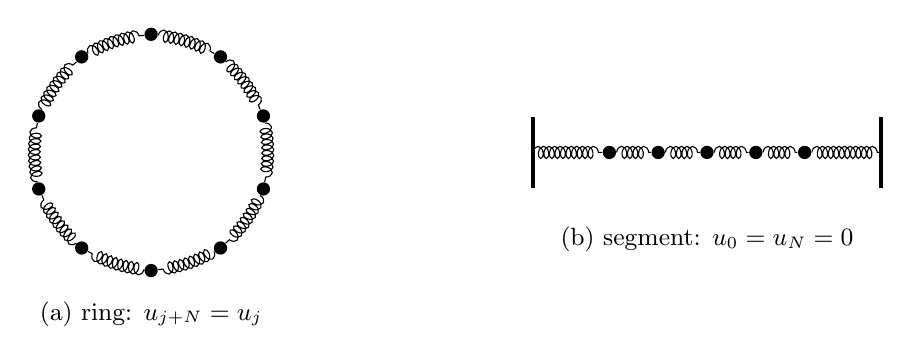
\begin{tikzpicture}[
  bead/.style={circle,fill=black,inner sep=1.7pt},
  spring/.style={decorate,decoration={coil,aspect=0.6,segment length=2pt,amplitude=2.2pt}}]
% (a) ring
\begin{scope}
  \def\R{1.5}
  \foreach \i in {0,...,9}{\node[bead] (b\i) at ({90-36*\i}:\R){};}
  \foreach \i [evaluate=\i as \j using {int(mod(\i+1,10))}] in {0,...,9}
    {\draw[spring] (b\i) to[bend left=10] (b\j);}
  \node at (0,-\R-0.55){\small (a) ring: $u_{j+N}=u_j$};
\end{scope}
% (b) segment
\begin{scope}[xshift=5.2cm,yshift=0cm]
  \draw[very thick] (-0.35,-0.45) -- (-0.35,0.45);
  \draw[very thick] ({6*0.62+0.35},-0.45) -- ({6*0.62+0.35},0.45);
  \foreach \i in {1,...,5}{\node[bead] (s\i) at (\i*0.62,0){};}
  \draw[spring] (-0.35,0) -- (s1);
  \foreach \i [evaluate=\i as \j using {int(\i+1)}] in {1,...,4}{\draw[spring] (s\i) -- (s\j);}
  \draw[spring] (s5) -- ({6*0.62+0.35},0);
  \node at ({3*0.62},-1.1){\small (b) segment: $u_0=u_N=0$};
\end{scope}
\end{tikzpicture}
\caption{The two geometries. (a) The ring of $N$ beads coupled by identical springs gives a
\emph{circulant} Laplacian $\LN=\circm(2,-1,0,\dots,0,-1)$. (b) The Dirichlet segment gives the
\emph{tridiagonal Toeplitz} $T_N=\operatorname{tridiag}(-1,2,-1)$. Both have the same symbol
$f(\theta)=4\sin^2(\theta/2)$.}\label{fig:chains}
\end{figure}

\subsection{Toeplitz, Hankel, circulant}
A matrix is \emph{Toeplitz} if it is constant along diagonals, $A_{ij}=a_{i-j}$ ($2n-1$ scalars,
$O(n)$ storage); \emph{Hankel} if constant along anti-diagonals, $H_{ij}=h_{i+j}$; and
\emph{circulant} if Toeplitz with a periodic wrap, $C_{ij}=c_{(i-j)\bmod n}$. For $n=4$,
\[
T=\begin{pmatrix}a_0&a_{-1}&a_{-2}&a_{-3}\\ a_1&a_0&a_{-1}&a_{-2}\\
a_2&a_1&a_0&a_{-1}\\ a_3&a_2&a_1&a_0\end{pmatrix},\quad
H=\begin{pmatrix}h_0&h_1&h_2&h_3\\ h_1&h_2&h_3&h_4\\ h_2&h_3&h_4&h_5\\ h_3&h_4&h_5&h_6\end{pmatrix},\quad
C=\begin{pmatrix}c_0&c_3&c_2&c_1\\ c_1&c_0&c_3&c_2\\ c_2&c_1&c_0&c_3\\ c_3&c_2&c_1&c_0\end{pmatrix}.
\]
Reversing rows turns Toeplitz into Hankel, $H=JT$ with $J$ the exchange matrix; a Toeplitz matrix is
the finite compression of a convolution (Laurent) operator. The ring Laplacian
$\LN=\circm(2,-1,0,\dots,0,-1)$ is the periodic case of the segment Toeplitz
$T_N=\operatorname{tridiag}(-1,2,-1)$.

\subsection{The symbol and circulant diagonalization}
A banded Toeplitz/circulant matrix with entries $a_k$ has \emph{symbol}
$f(\theta)=\sum_k a_k\eu^{\mathrm{i}k\theta}$; for both $\LN$ and $T_N$,
\[ f(\theta)=2-2\cos\theta=4\sin^2(\theta/2). \]
Every circulant is a polynomial $C=\sum_k c_k P^k$ in the cyclic shift $P$, and the Fourier modes
$\varphi^{(r)}_j=N^{-1/2}\eu^{2\pi\mathrm{i}rj/N}$ are common eigenvectors of $P$
($P\varphi^{(r)}=\eu^{2\pi\mathrm{i}r/N}\varphi^{(r)}$). Hence
\begin{equation}\label{eq:diag}
  \LN=F_N^\ast\Lambda F_N,\qquad
  \lambda_r=f\!\left(\tfrac{2\pi r}{N}\right)=4\sin^2\tfrac{\pi r}{N},\qquad
  \omega_r=\sqrt{\lambda_r}=2\sin\tfrac{\pi r}{N},
\end{equation}
$r=0,\dots,N-1$. The discrete dispersion relation $\omega(\theta)=2|\sin(\theta/2)|$ is literally the
square root of the symbol, sampled at $\theta=2\pi r/N$ on the ring and at $\theta=\pi k/(N{+}1)$ on
the segment ($\lambda^{\mathrm{Dir}}_k=4\sin^2\frac{\pi k}{2(N+1)}$). The twofold degeneracy
$\omega_r=\omega_{N-r}$ on the ring---absent on the segment---is the source of the arithmetic
difficulty in Section~\ref{sec:prime}.

\subsection{Classical Toeplitz algorithms}
Determined by $2n-1$ scalars, a Toeplitz system admits operations far below the dense $O(n^3)$
(Table~\ref{tab:toeplitz}); three enter the analysis.

\begin{table}[ht]\centering
\begin{tabular}{lll}
\toprule
Task & Algorithm & Cost \\
\midrule
Solve $Tx=b$ (symmetric) & Levinson (1947) & $O(n^2)$ \\
AR / Yule--Walker & Durbin (1960) & $O(n^2)$ \\
Inverse $T^{-1}$ (explicit) & Trench (1964) / Gohberg--Semencul (1972) & $O(n^2)$ \\
Multiply $Tx$, circulant solve, $f(\LN)$ & FFT / circulant embedding & $O(n\log n)$ \\
Semi-infinite chain & Wiener--Hopf factorization & --- \\
\bottomrule
\end{tabular}
\caption{Structured solvers used here; all beat the dense $O(n^3)$.}\label{tab:toeplitz}
\end{table}

\noindent\textbf{Levinson--Durbin.} For symmetric Toeplitz $R=(r_{|i-j|})$ the order-$i$ system
$R^{(i)}a^{(i)}=(r_1,\dots,r_i)^\top$ is built recursively through the \emph{reflection coefficients}
$k_i$ (PARCOR): with $E_0=r_0$,
\begin{equation}\label{eq:levinson}
  k_i=\frac{r_i-\sum_{j=1}^{i-1}a^{(i-1)}_j r_{i-j}}{E_{i-1}},\quad
  a^{(i)}_j=a^{(i-1)}_j-k_i\,a^{(i-1)}_{i-j},\quad a^{(i)}_i=k_i,\quad E_i=(1-k_i^2)E_{i-1}.
\end{equation}
Recursion~\eqref{eq:levinson} is due to Levinson~\cite{Levinson} and, in the AR (Yule--Walker) case,
Durbin~\cite{Durbin}; one has $|k_i|<1$ for all $i$ iff $R\succ0$, making $\{k_i\}$ the natural
stable-filter parametrization. The implementation used here goes back to the author's 2012
study~\cite{Gradina12} and is the AR core of the companion time-series work.

\noindent\textbf{Trench / Gohberg--Semencul.} The inverse of a Toeplitz matrix is \emph{not} Toeplitz
but is determined by its first and last columns $u,v$~\cite{Trench,GS} (two $O(n^2)$ recursions); writing $L_x,U_x$
for the lower/upper triangular Toeplitz matrices generated by a vector $x$,
\begin{equation}\label{eq:gs}
  T^{-1}=\tfrac1{u_0}\bigl(L_u U_{v}-L_{Sv}\,U_{Su}\bigr),
\end{equation}
a difference of products of triangular Toeplitz factors ($S$ the shift), with $\det T$ obtained en
route. On the ring this collapses to the pseudoinverse $\LN^{+}=F_N^\ast\Lambda^{+}F_N$ (the constant
mode, $\LN\mathbf1=0$, is mapped to $0$) and, more generally, $f(\LN)=F_N^\ast f(\Lambda)F_N$ in
$O(N\log N)$---the route by which the propagators below are evaluated.

\noindent\textbf{Wiener--Hopf.} On the semi-infinite chain the stiffness is a one-sided Toeplitz
operator; its inversion is the Wiener--Hopf factorization $f(\theta)=f_+(\theta)f_-(\theta)$ of the
symbol, which links the finite-$N$ ceilings to the operator-theoretic (Szeg\H{o}) asymptotics of
Section~\ref{sec:upper}.

\subsection{Three dynamics and the central functional}
The same lattice carries the wave equation $\ddot u+\LN u=0$ (propagator $\cos(t\sqrt{\LN})$), the
discrete Schr\"odinger equation $\mathrm i\dot z=\LN z$ (propagator $\eu^{-\mathrm i t\LN}$, the phase
governed by $\lambda_r$ rather than $\omega_r=\sqrt{\lambda_r}$), and the dissipative heat flow
$\dot v=-\LN v$ (no large wave---the semigroup smooths). For the wave equation with the unit zero-mean
velocity impulse $u(0)=0$, $\dot u(0)=e_0-\tfrac1N\mathbf 1$, the response is the velocity Green's
function
\begin{equation}\label{eq:green}
  u_j(t)=G_N(j,t)=\frac1N\sum_{r=1}^{N-1}\frac{\sin(\omega_r t)}{\omega_r}\,\eu^{2\pi\mathrm{i}rj/N}.
\end{equation}
As $u$ is real and $\omega_r=\omega_{N-r}$, \eqref{eq:green} is a real almost-periodic function of $t$
with frequency set $\{\omega_r\}$, and the large wave is the operator-norm growth
$A_N=\sup_t\max_j|G_N(j,t)|$.

\section{Bohr's supremum and the ceiling \texorpdfstring{$U_N$}{U\_N}}

\begin{proposition}[Bohr ceiling]\label{prop:bohr}
For every $N$ and every node $j$,
\(
  \sup_t|G_N(j,t)|\le U_N,\ U_N:=\tfrac1{2N}\sum_{r=1}^{N-1}\csc(\pi r/N),
\)
with equality at $j=0$ provided the frequencies $\{\omega_r:1\le r\le\lfloor N/2\rfloor\}$ are
linearly independent over $\Q$.
\end{proposition}

\begin{proof}
Grouping the degenerate pair $r,\,N-r$ gives, at $j=0$,
$G_N(0,t)=\sum_{r=1}^{\lfloor N/2\rfloor}b_r\sin(\omega_r t)$ with $b_r=2/(N\omega_r)>0$
(the term $r=N/2$, if present, has coefficient $1/(N\omega_{N/2})$). The triangle inequality
gives $|G_N(j,t)|\le\frac1N\sum_{r=1}^{N-1}\omega_r^{-1}=U_N$ for all $j$. If the $\omega_r$ are
$\Q$-independent, then by Kronecker--Weyl the orbit $\{(\omega_r t)_r\}$ is dense in the torus, so
$\sin(\omega_r t)\to1$ simultaneously and the bound is attained at $j=0$. (Bohr's theorem:
$\sup_t\sum b_r\sin(\omega_r t)=\sum|b_r|$.)
\end{proof}

\section{The exact constant}

\begin{lemma}[Euler--Maclaurin asymptotics]\label{lem:asym}
$\displaystyle U_N=\frac1\pi\Big(\ln N+\gamma+\ln\frac2\pi\Big)+o(1)
   =\frac1\pi\ln N+0.039\,99\ldots+o(1).$
\end{lemma}

\noindent The leading term comes from the singularity $\csc(\pi r/N)\sim N/(\pi r)$ at small $r$,
which yields the harmonic sum $\sum 1/r\sim\ln$; the constant follows from the Euler--Maclaurin
correction. Numerically $U_N-\tfrac1\pi\ln N\to0.03999$ for $N\le 65536$
(\texttt{numerics/verify\_lemma3\_lebesgue.py}).

\section{Upper bounds: energy and the Szeg\H{o} symbol}\label{sec:upper}

A fixed-energy bound caps the response. With energy
$E=\tfrac12\dot u^\top\dot u+\tfrac12 u^\top\LN u$ and the exact trigonometric identity (the cotangent
sum, derived in Section~\ref{sec:zeta})
\begin{equation}\label{eq:csc2}
  \sum_{r=1}^{N-1}\frac1{\sin^2(\pi r/N)}=\frac{N^2-1}{3},
\end{equation}
Cauchy--Schwarz on the modal expansion gives $\|u(t)\|_\infty\le C\sqrt N\,\sqrt E$: at fixed energy
the deflection cannot exceed order $\sqrt N$, a ceiling attained by the time-reversed focusing
configuration (the variational maximum; \texttt{verify\_theorem1.py}). The same sum yields the exact
pseudo-inverse diagonal $(\LN^{+})_{jj}=\tfrac1N\sum_{r\ne0}\lambda_r^{-1}=\tfrac{N^2-1}{12N}$.

Asymptotically the eigenvalues follow the symbol through Szeg\H{o}'s theorem~\cite{GrenanderSzego,Gray}:
for continuous $F$,
\begin{equation}\label{eq:szego}
  \frac1N\sum_{r=0}^{N-1}F(\lambda_r)\xrightarrow{N\to\infty}\frac1{2\pi}\int_0^{2\pi}F\bigl(f(\theta)\bigr)\,d\theta,
  \qquad f(\theta)=4\sin^2(\theta/2),
\end{equation}
so spectral sums such as $U_N$ and $(\LN^{+})_{jj}$ are Riemann sums of the symbol; the logarithmic
growth of $U_N$ is exactly the borderline (logarithmically divergent) singularity
$f^{-1/2}\sim|\theta|^{-1}$ at $\theta=0$. (Szeg\H{o}'s theorem
proper requires continuous $F$; the \emph{singular} sums $U_N=\tfrac1{2N}\sum\lambda_r^{-1/2}$ and
$(\LN^{+})_{jj}=\tfrac1N\sum\lambda_r^{-1}$ are made rigorous by Euler--Maclaurin at the band edge,
Appendix~\ref{app:bernoulli}, the singularity producing the logarithm and the $N^2$ growth.) The propagators
$\cos(t\sqrt{\LN})$, $\eu^{-\mathrm i t\LN}$, $\LN^{-1/2}\sin(t\sqrt{\LN})$ are functions of the matrix
in the sense of Golub--Van Loan~\cite{GVL}, evaluated exactly by \eqref{eq:diag}; this puts the
operator-norm functionals $\|f_t(\LN)\|_{\ell^p\to\ell^q}$ on a rigorous footing.

\section{The spectral zeta function and the large-wave constants}\label{sec:zeta}

Define the spectral zeta of the ring Laplacian (zero mode removed),
\begin{equation}\label{eq:zeta}
  \zeta_{\LN}(s)=\sum_{r=1}^{N-1}\lambda_r^{-s}=4^{-s}\sum_{r=1}^{N-1}\csc^{2s}\tfrac{\pi r}{N},
  \qquad \Re s>0 .
\end{equation}
At integer $s$ this is a cosecant power sum with a closed form in $N$ (Bernoulli numbers,
Appendix~\ref{app:bernoulli}); the first two are
\[
  \zeta_{\LN}(1)=\frac{N^2-1}{12},\qquad \zeta_{\LN}(2)=\frac{(N^2-1)(N^2+11)}{720}.
\]
The first is elementary: from the classical identity $\sum_{r=1}^{N-1}\cot^2\frac{\pi r}{N}=\frac{(N-1)(N-2)}3$
and $\csc^2=1+\cot^2$,
\[
  \sum_{r=1}^{N-1}\csc^2\tfrac{\pi r}{N}=(N-1)+\frac{(N-1)(N-2)}3=\frac{N^2-1}3,
  \qquad\text{so}\qquad \zeta_{\LN}(1)=\tfrac14\sum_{r}\csc^2\tfrac{\pi r}{N}=\frac{N^2-1}{12},
\]
and $\zeta_{\LN}(2)$ follows the same way from $\sum_r\csc^4=\frac{(N^2-1)(N^2+11)}{45}$ (all integer values
are even polynomials in $N$, \texttt{verify\_spectral\_zeta.py}).
The two large-wave constants are \emph{special values of this single object}:
\begin{equation}\label{eq:zeta-values}
  U_N=\frac{\zeta_{\LN}(1/2)}{N},\qquad M_N^2=\frac{2E_0\,\zeta_{\LN}(1)}{N},
\end{equation}
the first because $\csc(\pi r/N)=2\lambda_r^{-1/2}$, the second because $(\LN^{+})_{jj}=\zeta_{\LN}(1)/N$.
Thus the Bohr ceiling (the large wave, $A_N\sim U_N$) and the variational ceiling $M_N$
(Section~\ref{sec:upper}) are the values of $\zeta_{\LN}$ at $s=\tfrac12$ and $s=1$.

The two growth laws are then dictated by the analytic structure of $\zeta_{\LN}$. By Szeg\H{o}'s
theorem the normalized zeta converges to the symbol integral,
\begin{equation}\label{eq:zeta-density}
  \frac1N\,\zeta_{\LN}(s)\xrightarrow{N\to\infty}
  I(s)=\frac1{2\pi}\int_0^{2\pi}(2-2\cos\theta)^{-s}\,d\theta
  =\frac{4^{-s}\,\Gamma(\tfrac12-s)}{\sqrt{\pi}\,\Gamma(1-s)},\qquad \Re s<\tfrac12,
\end{equation}
which has a simple pole at $s=\tfrac12$ (Figure~\ref{fig:zeta}). The edge of convergence is exactly the
logarithmic singularity producing $U_N=\zeta_{\LN}(\tfrac12)/N=\tfrac1\pi\ln N+O(1)$ (Lemma~\ref{lem:asym}).
At $s=1$ the density diverges, and indeed $\zeta_{\LN}(1)\sim N^2/12$ yields the $\sqrt N$ variational
ceiling $M_N\sim\sqrt{N/6}$. \emph{The large wave sits precisely at the convergence edge $s=\tfrac12$ of
the limiting spectral density $I(s)$}; the finite-$N$ $\zeta_{\LN}$ is itself an entire finite sum, and
it is the $N\to\infty$ density that carries the pole. The finite-$N$ zeta is an Epstein/Hurwitz-type
object whose integer values are polynomials in $N^2$ and whose half-integer value carries the logarithm.
All identities are verified (\texttt{verify\_spectral\_zeta.py}). At the opposite end, the spectral
determinant is the $s=0$ \emph{derivative}: $\zeta_{\LN}'(0)=-\log\det{}'\LN$ with
$\det{}'\LN=\prod_{r\ne0}\lambda_r=N^2$ (from $\prod_{r=1}^{N-1}2\sin(\pi r/N)=N$), so by Kirchhoff's
matrix-tree theorem the cycle $C_N$ has exactly $\det{}'\LN/N=N$ spanning trees---a graph invariant read
off $\zeta_{\LN}'(0)$ (\texttt{verify\_spanning\_trees.py}).

\begin{figure}[ht]\centering

\includegraphics[width=.72\textwidth]{fig_zeta.pdf}
\caption{The normalized spectral zeta $\frac1N\zeta_{\LN}(s)$ converges to the symbol density $I(s)$ of
\eqref{eq:zeta-density}, which has a pole at $s=\tfrac12$. The large-wave ceiling is the boundary value
$U_N=\zeta_{\LN}(\tfrac12)/N\sim\tfrac1\pi\ln N$.}\label{fig:zeta}
\end{figure}

\section{Operator-norm hierarchy and the variational principle}\label{sec:opnorm}

The large wave is one corner of a hierarchy of operator norms of the velocity propagator
$S_N(t)=f_t(\LN)$ on the zero-mean subspace $\mathcal H_0=\{x\in\R^N:\sum_jx_j=0\}$, where
$f_t(\lambda)=\sin(t\sqrt\lambda)/\sqrt\lambda$ for $\lambda>0$ and $f_t(0)=0$ (circulant on
$\mathcal H_0$, kernel $G_N$; the constant mode is excluded since $\LN\mathbf1=0$). Its time-supremum in
different $\ell^p\to\ell^q$ norms obeys \emph{three distinct growth laws} (Table~\ref{tab:opnorm}, all
verified by \texttt{verify\_operator\_norms.py}):
\begin{equation}\label{eq:opnorm}
\begin{aligned}
  \sup_t\|S_N(t)\|_{2\to2}&=\frac1{2\sin(\pi/N)}\sim\frac{N}{2\pi},\\
  \sup_t\|S_N(t)\|_{2\to\infty}&\le\sqrt{\tfrac{\zeta_{\LN}(1)}{N}}\sim\sqrt{\tfrac N{12}},\\
  \sup_t\|S_N(t)\|_{1\to\infty}&=A_N\le U_N\sim\tfrac1\pi\ln N .
\end{aligned}
\end{equation}
\emph{Derivations.} $S_N(t)$ is symmetric with eigenvalues $f_t(\lambda_r)=\sin(t\omega_r)/\omega_r$, so
its $\ell^2\!\to\!\ell^2$ norm is $\max_r|\sin(t\omega_r)|/\omega_r$, whose supremum over $t$ is
$1/\omega_1=1/(2\sin\tfrac\pi N)$---the slowest mode reaching $\sin(t\omega_1)=\pm1$; this is exact and
unconditional. For $\ell^2\!\to\!\ell^\infty$, by translation invariance the norm is the $\ell^2$-length
of one row of $G_N$, and Parseval gives
\[
  \|G_N(\cdot,t)\|_2^2=\frac1N\sum_{r=1}^{N-1}\frac{\sin^2(t\omega_r)}{\omega_r^2}
  \ \le\ \frac1N\sum_{r}\omega_r^{-2}=\frac{\zeta_{\LN}(1)}N,
\]
hence $\sup_t\|S_N(t)\|_{2\to\infty}\le\sqrt{\zeta_{\LN}(1)/N}\sim\sqrt{N/12}$, with equality iff all
$\sin^2(t\omega_r)=1$ simultaneously---rational independence ($N$ prime, $2^m$). Finally
$\|S_N(t)\|_{1\to\infty}=\max_{j,k}|S_N(t)_{jk}|=\max_m|G_N(m,t)|$, whose time-supremum is, by definition,
$A_N\le\sum_r|a_r|=U_N$. The three corners thus read the spectral sums $\sum_r\omega_r^{-p}$ ($p=1,2$)
through different lenses; the $\ell^1\!\to\!\ell^\infty$ corner---weakest input, strongest output---is
precisely the large wave $A_N$.

\emph{Variational principle.} The energy norm has the direct reading: maximizing the deflection at a
node over the energy sphere $E(u_0,v_0)\le E_0$ on $\mathcal H_0$ is a constrained quadratic problem solved by Lagrange
multipliers,
\[
  \sup_{E(u_0,v_0)\le E_0}\ \max_j|u_j(t)| = \sqrt{2E_0\,(\LN^{+})_{jj}}=\sqrt{\tfrac{E_0(N^2-1)}{6N}}=M_N,
\]
\emph{independent of $t$} (the focusing configuration is the time-reversed peak). This is the
operator-norm/variational face of the energy ceiling, and via \eqref{eq:zeta-values} both $M_N$ and
$U_N$ are special values of the spectral zeta. The Szeg\H{o} symbol $f(\theta)=4\sin^2(\theta/2)$
controls all three norms through the spectral sums $\sum_r\omega_r^{-p}$.

\begin{table}[ht]\centering
\begin{tabular}{llll}
\toprule
norm & $\sup_t\|S_N(t)\|$ & growth & meaning \\
\midrule
$\ell^2\!\to\!\ell^2$ & $1/(2\sin\tfrac\pi N)$ & $N/2\pi$ & lowest-mode resonance \\
$\ell^2\!\to\!\ell^\infty$ & $\le\sqrt{\zeta_{\LN}(1)/N}$ & $\sqrt{N/12}$ & energy ceiling / variational $M_N$ \\
$\ell^1\!\to\!\ell^\infty$ & $A_N\le U_N=\zeta_{\LN}(1/2)/N$ & $\tfrac1\pi\ln N$ & \textbf{large wave} $A_N$ \\
\bottomrule
\end{tabular}
\caption{Three growth laws from one propagator. The $\ell^2\!\to\!\ell^2$ supremum is exact and
unconditional; the other two equal the listed ceilings on the $\Q$-independent classes $N$ prime and
$N=2^m$ (for $N=2p$, Proposition~\ref{prop:2p} gives only an $O(N^{-1})$ gap for the
$\ell^1\!\to\!\ell^\infty$ large wave) and are bounded by them in general. The large wave is the
$\ell^1\!\to\!\ell^\infty$ corner.}\label{tab:opnorm}
\end{table}

\section{Independence theorems and unconditional growth}\label{sec:prime}

\begin{theorem}[odd prime]\label{thm:prime}
Let $p$ be an odd prime. Then $\{\sin(\pi r/p):1\le r\le\tfrac{p-1}2\}$ is linearly independent
over $\Q$; hence $A_p=U_p\sim\tfrac1\pi\ln p$.
\end{theorem}

\begin{proof}
Put $\eta=\zeta_{2p}=\eu^{\mathrm{i}\pi/p}$. As $p$ is odd, $[\Q(\eta):\Q]=\varphi(2p)=p-1$, so
$\{1,\eta,\dots,\eta^{p-2}\}$ is a $\Q$-basis, and $\eta^{p}=\eu^{\mathrm{i}\pi}=-1$. From
$\eta^{-r}=\eta^{2p-r}=\eta^{p}\eta^{p-r}=-\eta^{p-r}$ we get $2\mathrm{i}\sin(\pi r/p)=\eta^r-\eta^{-r}=\eta^r+\eta^{p-r}$.
Suppose $\sum_{r=1}^{(p-1)/2}c_r\sin(\pi r/p)=0$ with $c_r\in\Q$. Then
$\sum_r c_r\eta^r+\sum_r c_r\eta^{p-r}=0$. As $r$ runs over $\{1,\dots,\tfrac{p-1}2\}$ the exponents
$r$ fill $\{1,\dots,\tfrac{p-1}2\}$ and $p-r$ fill $\{\tfrac{p+1}2,\dots,p-1\}$, together covering
$\{1,\dots,p-1\}$ bijectively, so $\sum_{m=1}^{p-1}d_m\eta^m=0$ with $d_m=c_m$ or $c_{p-m}$.
Finally $\Phi_{2p}(\eta)=\sum_{j=0}^{p-1}(-1)^j\eta^j=0$ gives $\eta^{p-1}=-\sum_{j=0}^{p-2}(-1)^j\eta^j$,
whose constant term is $-1\ne0$; equating coordinates in $\{1,\eta,\dots,\eta^{p-2}\}$ forces
$d_{p-1}=0$ and then all $d_m=0$, i.e. all $c_r=0$. The conclusion follows from
Proposition~\ref{prop:bohr}. \end{proof}

\begin{theorem}[powers of two]\label{thm:two}
For $N=2^m$, $\{\sin(\pi r/N):1\le r\le N/2\}$ is $\Q$-independent; hence $A_N=U_N\sim\tfrac1\pi\ln N$.
\end{theorem}

\begin{proof}
Now $\eta=\zeta_{2N}$, $\Phi_{2N}(x)=x^{N}+1$ (degree $\varphi(2N)=N$), so $\{1,\dots,\eta^{N-1}\}$ is a
basis and $\eta^{N}=-1$. Again $2\mathrm{i}\sin(\pi r/N)=\eta^r+\eta^{N-r}$, and for $1\le r\le N/2$ the
exponents $r$ and $N-r$ lie in $\{1,\dots,N-1\}$ \emph{without reduction}; they are distinct basis
powers (the index $N/2$ occurring with coefficient $2c_{N/2}$). Linear independence is immediate.
\end{proof}

An exact integer-rank certificate validates the prime case (\texttt{verify\_lemma1\_prime.py}); the
general rank formula is checked separately by \texttt{verify\_independence\_rank.py}.

\medskip\noindent\textbf{Worked example (prime $N=5$).} The two distinct frequencies
$\omega_1=2\sin36^\circ=1.1756$ and $\omega_2=2\sin72^\circ=1.9021$ stand in the ratio
$\omega_2/\omega_1=2\cos36^\circ=\varphi=\tfrac{1+\sqrt5}2$, the \emph{golden ratio}---irrational, so the
relation lattice is trivial ($\Lambda_5=\{0\}$) and Theorem~\ref{thm:prime} applies. The node-$0$ response
is the two-tone signal $G_5(0,t)=\tfrac25\bigl(\omega_1^{-1}\sin\omega_1 t+\omega_2^{-1}\sin\omega_2 t\bigr)$,
and by Kronecker both sines reach $1$ at a common near-alignment time, so
\[
  A_5=U_5=\tfrac15\bigl(\csc36^\circ+\csc72^\circ\bigr)=0.5506,
\]
the supremum equal to the ceiling, approached arbitrarily closely (in contrast to the composite $N=12$ below;
\texttt{verify\_exact\_AN.py}).

\begin{observation}[low-mode prefix]\label{obs:prefix}
Let $M(N)$ be the largest $M$ with $\{\sin(\pi r/N):r\le M\}$ $\Q$-independent; by Kronecker these modes
can be brought simultaneously into phase, contributing
$L_{\mathrm{pre}}(N)=\tfrac1N\sum_{r=1}^{M(N)}\csc(\pi r/N)$, which numerically satisfies
$L_{\mathrm{pre}}(N)\ge 0.25\,\ln N$ for all tested $N\le256$ (including the highly composite
$N=210,240$). This does \emph{not} by itself bound $A_N$ from below: the out-of-prefix modes may
interfere destructively, and controlling that interference is the open step.
\end{observation}

\begin{conjecture}[order, all $N$]\label{conj:order}
$A_N=\Theta(\ln N)$ for every $N$; more precisely $A_N\sim\tfrac1\pi\ln N$. This is proved for $N$ prime,
$N=2^m$, and $N=2p$ (Theorems~\ref{thm:prime}--\ref{thm:two}, Proposition~\ref{prop:2p}); for general
$N$ it is supported by Observation~\ref{obs:prefix} and by the exact subtorus computation of
Section~\ref{sec:exact}, where $A_N/\ln N$ stays in $[0.28,0.31]$ throughout the tested range
(\texttt{verify\_lemma4\_prefix.py}, \texttt{verify\_open\_problems.py}), but is not proved. The exact
saturation locus $A_N=U_N$ is settled by the arithmetic criterion of Theorem~\ref{thm:ceiling}; the open
content is the \emph{lower} order of $A_N$ on the non-saturating $N$.
\end{conjecture}

\subsection{The Dirichlet segment}\label{sub:segment}
The segment chain $\mathrm{tridiag}(-1,2,-1)$ with Dirichlet ends has the \emph{simple} spectrum
$\mu_k=2\sin\frac{\pi k}{2(N+1)}$ ($k=1,\dots,N$): no degeneracy, the structural advantage over the
ring, whose twofold $\mu_r=\mu_{N-r}$ halves the independent phases. Writing $\mu_k=2\sin(2\pi k/M)$ with
$M=4(N+1)$, the frequencies lie in $\Q(\zeta_M)$ with $2\mathrm{i}\sin(2\pi k/M)=\zeta_M^k-\zeta_M^{-k}$,
and the same minus-eigenspace argument gives the subtorus dimension
\begin{equation}\label{eq:segrank}
  \dim_\Q\operatorname{span}\{\mu_1,\dots,\mu_N\}=\min\!\bigl(N,\ \tfrac12\varphi(4(N+1))\bigr)
  \qquad(\text{verified for }N\le30,\ \text{conjectured in general}),
\end{equation}
which is full ($=N$, whence $A_N^{\mathrm{Dir}}=U_N^{\mathrm{Dir}}\sim\frac1\pi\ln N$ by Bohr)
when $N+1$ is prime or a power of two (and, assuming \eqref{eq:segrank}, only then)---the exact analogue of Theorems~\ref{thm:prime}--\ref{thm:two}
shifted by the boundary (the ring uses modulus $2N$, the segment $4(N+1)$). The $\Q$-independent low-mode
prefix again supports $A_N^{\mathrm{Dir}}=\Theta(\ln N)$ for every $N$ numerically, subject to the same
out-of-prefix gap as Conjecture~\ref{conj:order} (\texttt{verify\_segment\_lower\_bound.py}).

\section{Exact \texorpdfstring{$A_N$}{A\_N} for composite \texorpdfstring{$N$}{N}}\label{sec:exact}

For composite $N$ the frequencies satisfy rational relations and the orbit closure is a proper
\emph{subtorus} (Weyl). In the cyclotomic coordinates $C$ (row $r$ = integer coordinates of
$2\mathrm{i}\sin(\pi r/N)$ in $\Q(\zeta_{2N})$) the attainable phases are $\{\varphi=C\psi\}$, whence
\begin{equation}\label{eq:subtorus}
  \sup_t u_j(t)=\max_{\psi\in\R^p}\sum_r a_{rj}\sin\big((C\psi)_r\big),\qquad p=\varphi(2N),
\end{equation}
a finite-dimensional trigonometric maximization, reduced exactly and then evaluated numerically
(\texttt{verify\_exact\_AN.py}, returning $A_N=U_N$ on primes; a certified global bracket is given for
$N=6$ below). This makes the composite case computable for each $N$:
numerically the subtorus defect on the ring is $A_N/U_N\in[0.84,0.92]$ in the tested range, so
$A_N/\ln N\in[0.28,0.31]$, consistent with Conjecture~\ref{conj:order} ($A_N=\Theta(\ln N)$).

\begin{proposition}[algebraic composite cases]\label{prop:closed}
$A_N$ is an algebraic number: writing $x_r=\cos\varphi_r$, $y_r=\sin\varphi_r$ with $x_r^2+y_r^2=1$ and
adjoining, for each generator $k$ of the relation lattice $\Lambda$, the constraints
$\cos\langle k,\varphi\rangle=1$, $\sin\langle k,\varphi\rangle=0$ that cut out the orbit-closure subtorus
$\mathbb{T}_N$ (polynomials in the $x_r,y_r$ through the Chebyshev/addition formulas), turns
\eqref{eq:subtorus} into the maximum of a polynomial over a compact semialgebraic set defined over $\Q$,
whose value is algebraic by the Tarski--Seidenberg theorem (real quantifier elimination). For $N=6$ the relation lattice is one-dimensional and
\[
  A_6=\frac{\sqrt3}{9}+\frac{(3+\sqrt3)\,\sqrt[4]{3}}{12\sqrt2}\approx0.55942 ,
\]
with the inner maximum at $\cos\varphi=(\sqrt3-1)/2$. For $N=12$ the three-term relation
$\omega_5=\omega_1+\omega_3$ (i.e. $\sin75^\circ-\sin15^\circ=\sin45^\circ$) makes the block
two-dimensional; the algebraic degree grows with the arithmetic of $N$, and no uniform elementary
closed form is apparent.
\end{proposition}

\medskip\noindent\textbf{Worked example ($N=12$).} The six distinct frequencies $\omega_r=2\sin(\pi r/12)$
are
\[
  (\omega_1,\dots,\omega_6)=\bigl(2\sin15^\circ,\ 1,\ \sqrt2,\ \sqrt3,\ 2\sin75^\circ,\ 2\bigr)
  \approx(0.518,\ 1,\ 1.414,\ 1.732,\ 1.932,\ 2),
\]
and their relation lattice $\Lambda_{12}$ is rank two, generated by
\[
  \omega_5=\omega_1+\omega_3\quad(2\sin75^\circ-2\sin15^\circ=\sqrt2),\qquad
  \omega_6=2\omega_2\quad(2=2\cdot1).
\]
Both generators have coefficient-sum $\not\equiv0\ (\mathrm{mod}\ 4)$---reading
$\omega_5-\omega_1-\omega_3=0$ as $-1-1+1\equiv3$ and $2\omega_2-\omega_6=0$ as $2-1\equiv1$---so by the
criterion below (Theorem~\ref{thm:ceiling}) the ceiling is \emph{not} attained, $A_{12}<U_{12}$. Solving
the subtorus maximization~\eqref{eq:subtorus} numerically gives
\[
  U_{12}=\tfrac1{24}\sum_{r=1}^{11}\csc\tfrac{\pi r}{12}=0.8307,\qquad A_{12}=0.7546,\qquad
  \frac{A_{12}}{U_{12}}=0.908 ,
\]
the two relations pulling the optimal phases off $\varphi_r=\tfrac\pi2$ by just enough to cost $9\%$ of the
ceiling (\texttt{verify\_relation\_lattices.py}, \texttt{verify\_exact\_AN.py}).

A sharp arithmetic criterion decides exactly when the ceiling is reached.

\begin{theorem}[ceiling criterion]\label{thm:ceiling}
Let $\Lambda=\{k\in\Z^m:\sum_r k_r\omega_r=0\}$ be the relation lattice of the distinct positive
frequencies $\omega_r=2\sin(\pi r/N)$, $1\le r\le m=\lfloor N/2\rfloor$. Then $A_N=U_N$ if and only if
\[
  \sum_{r}k_r\equiv0\ (\mathrm{mod}\ 4)\quad\text{for every }k\in\Lambda
\]
or, when $N$ is even, the antipodal variant $\sum_r k_r+2\sum_r rk_r\equiv0\ (\mathrm{mod}\ 4)$ holds for
every $k\in\Lambda$. The two conditions coincide for all $N\le160$ (where only $N$ prime and $N=2^m$
saturate, Corollary~\ref{cor:density}).
\end{theorem}

\begin{proof}
Always $A_N\le U_N$, with $U_N=\sum_r a_{r0}$ the node-$0$ ceiling. As $a_{rj}=a_{r0}\cos(2\pi rj/N)$ we
have $|a_{rj}|\le a_{r0}$, so no node exceeds $U_N$, and $|a_{rj}|=a_{r0}$ for \emph{all} $r$ forces
$|\cos(2\pi rj/N)|=1$, i.e.\ $2j/N\in\Z$: only $j=0$ and---for even $N$---$j=N/2$ can attain the ceiling.
At $j=0$ the coefficients $a_{r0}>0$, so $U_N$ is reached iff all $\sin(\omega_r t)$ can be driven to $1$
simultaneously, i.e.\ the target $\varphi_\ast=(\tfrac\pi2,\dots,\tfrac\pi2)$ lies in the orbit closure
$\mathbb{T}_N$. By Kronecker, $\varphi_\ast\in\mathbb{T}_N$ iff $\langle k,\varphi_\ast\rangle=
\tfrac\pi2\sum_r k_r\equiv0\ (2\pi)$ for every $k\in\Lambda$, i.e.\ $\sum_r k_r\equiv0\ (4)$. At $j=N/2$
(even $N$) the signs $\cos(\pi r)=(-1)^r$ give the alternating target $\varphi_r=\tfrac\pi2+\pi r$, and the
same argument yields $\langle k,\varphi\rangle=\tfrac\pi2\sum_r k_r+\pi\sum_r rk_r\equiv0\ (2\pi)$, i.e.\
$\sum_r k_r+2\sum_r rk_r\equiv0\ (4)$. The ceiling is attained iff one of the two admissible nodes
realizes its target, giving the stated disjunction (\texttt{verify\_ceiling\_criterion.py}).
\end{proof}

This refines the independence test: $\Q$-independence means $\Lambda=\{0\}$, which satisfies the
criterion vacuously, recovering $A_N=U_N$ for $N$ prime and $N=2^m$. The criterion is genuinely weaker in
principle---a composite $N$ with dependent frequencies could still saturate, provided every relation has
coefficient-sum divisible by $4$. Computing $\Lambda$ exactly by integer (Hermite) reduction of the
cyclotomic coordinates and testing the criterion against the directly optimized $A_N/U_N$, the two
agree for all $N\le40$, and a criterion-only scan finds \emph{no} composite $N\le160$ that saturates:
on this range $A_N=U_N$ holds precisely for $N$ prime or $N=2^m$ (\texttt{verify\_ceiling\_criterion.py}).
The \emph{full-independence} route to saturation is in fact closed for \emph{all} $N$ by
Theorem~\ref{thm:qrank} ($\operatorname{rank}=\tfrac12\varphi(2N)=\lfloor N/2\rfloor$ only for prime and
$2^m$, confirmed numerically to $N\le500$, \texttt{verify\_order\_extended.py}); a composite saturator
would have to satisfy the mod-$4$ criterion \emph{despite} rational dependence, which none $\le160$ does.
Table~\ref{tab:lattices} makes the lattices explicit; e.g.\ the generators
$\omega_3=2\omega_1$ ($N=6$), $\omega_5=\omega_1+\omega_3$ ($N=12$, cf.\ Proposition~\ref{prop:closed}),
and $\omega_4+\omega_5=\omega_1+2\omega_2+\omega_3$ ($N=15$) all have coefficient-sum $\not\equiv0\ (4)$.

\begin{table}[ht]\centering
\caption{Relation lattices $\Lambda_N$ of the distinct frequencies $\omega_r$ and the mod-4 criterion.
Primes and powers of two have $\Lambda_N=\{0\}$ and saturate; every composite $N$ listed carries a
relation with coefficient-sum $\not\equiv0\ (\mathrm{mod}\ 4)$, hence $A_N<U_N$; for even $N$ the
antipodal sums $\sum_r k_r+2\sum_r rk_r$ are violated likewise (\texttt{verify\_ceiling\_criterion.py},
check~E).}\label{tab:lattices}
\begin{tabular}{rlccl c}
\toprule
$N$ & class & \#freq & $\operatorname{rank}\Lambda_N$ & coeff-sums $\bmod\,4$ & $A_N=U_N$?\\
\midrule
$5$ & prime & $2$ & $0$ & --- & yes\\
$6$ & composite & $3$ & $1$ & $3$ & no\\
$8$ & $2^m$ & $4$ & $0$ & --- & yes\\
$9$ & composite & $4$ & $1$ & $3$ & no\\
$10$ & composite & $5$ & $1$ & $1$ & no\\
$12$ & composite & $6$ & $2$ & $3,3$ & no\\
$15$ & composite & $7$ & $3$ & $2,3,3$ & no\\
$16$ & $2^m$ & $8$ & $0$ & --- & yes\\
$18$ & composite & $9$ & $3$ & $3,3,3$ & no\\
$20$ & composite & $10$ & $2$ & $1,1$ & no\\
$21$ & composite & $10$ & $4$ & $1,3,3,3$ & no\\
$24$ & composite & $12$ & $4$ & $3,3,3,3$ & no\\
\bottomrule
\end{tabular}
\end{table}

\begin{corollary}[saturating families and a finite scan]\label{cor:density}
The two proven saturating families, the primes and the powers of two, both have natural density zero.
An exhaustive criterion scan finds no further saturating $N\le160$, so on this range
$\{N:A_N=U_N\}=\{N\text{ prime}\}\cup\{2^m\}$. Whether any composite $N$ saturates at all---and hence
whether the saturating set is genuinely of density zero---remains open, decided for each $N$ by
Theorem~\ref{thm:ceiling}.
\end{corollary}

\medskip\noindent\textbf{The composite gap.} For every composite $N\le160$, then, $A_N<U_N$. The gap is
\emph{certified} for $N=6$: the lone relation $2\omega_1=\omega_3$ has coefficient-sum
$2+0-1\equiv3\ (4)\ne0$, so by Theorem~\ref{thm:ceiling} $A_6<U_6$; quantitatively a Lipschitz-grid
certificate on the two-dimensional subtorus---the elementary level of the Lasserre moment--SOS
hierarchy~\cite{Lasserre}---brackets $A_6\in[0.5594,0.5604]$, so $U_6-A_6\ge0.048>0$, while the prime
$N=5$ returns $A_5=U_5$ (\texttt{verify\_sos\_certified.py}).

\begin{proposition}[twice a prime: the sharp constant on a composite family]\label{prop:2p}
For $N=2p$ with $p$ an odd prime, $A_N=U_N-O(1/N)=\tfrac1\pi\ln(2p)+O(1)$; the sharp constant $1/\pi$
holds, extending Theorems~\ref{thm:prime}--\ref{thm:two} to an infinite family of \emph{composite} $N$.
\end{proposition}

\begin{proof}
The prefix $\{\omega_1,\dots,\omega_{p-1}\}=\{2\sin(\pi r/2p):1\le r\le p-1\}$ is $\Q$-independent: in
$\Q(\zeta_{4p})$, where $\Phi_{4p}(x)=\Phi_p(-x^2)$ has degree $\varphi(4p)=2(p-1)$, the values
$2\mathrm i\sin(\pi r/2p)=\zeta_{4p}^{\,r}-\zeta_{4p}^{-r}$ ($1\le r\le p-1$) are linearly independent over
$\Q$. Indeed, if $\sum_{r=1}^{p-1}c_r(\zeta_{4p}^{\,r}-\zeta_{4p}^{-r})=0$ with $c_r\in\Q$, multiplying by
$\zeta_{4p}^{\,p-1}$ gives $Q(\zeta_{4p})=0$, where $Q(x)=\sum_{r=1}^{p-1}c_r(x^{p-1+r}-x^{p-1-r})$ has
degree $\le2p-2=\deg\Phi_{4p}$; as $\Phi_{4p}$ is the minimal polynomial of $\zeta_{4p}$, this forces
$Q=C\,\Phi_{4p}$, but $Q(1)=0$ while $\Phi_{4p}(1)=\Phi_p(-1)=1$, so $C=0$ and $Q\equiv0$, and since the
exponent sets $\{p-1+r\}_r$ and $\{p-1-r\}_r$ are disjoint, every $c_r=0$ (exact integer rank $=p-1$,
\texttt{verify\_2p\_family.py}). Thus the sole $\Q$-dependent frequency is the rational $\omega_p=2$, of
weight $\tfrac1{2N}$. With the degeneracy
$\omega_r=\omega_{N-r}$ the node-$0$ response is
$u_0(t)=\tfrac2N\sum_{r=1}^{p-1}\omega_r^{-1}\sin(\omega_r t)+\tfrac1{2N}\sin 2t$. By Kronecker the
independent prefix can be driven to $\sin(\omega_r t)\to1$ simultaneously, and since
$\tfrac2N\sum_{r=1}^{p-1}\omega_r^{-1}=\tfrac1N\sum_{r=1}^{p-1}\csc\tfrac{\pi r}{2p}=U_N-\tfrac1{2N}$,
we get $\sup_t u_0(t)\ge U_N-\tfrac1N$. As $A_N\le U_N$ always, $A_N\in[U_N-\tfrac1N,\,U_N]$
(\texttt{verify\_2p\_family.py}).
\end{proof}

\begin{figure}[ht]\centering

\includegraphics[width=.78\textwidth]{fig_ring.pdf}
\caption{Ring large wave $A_N$ versus $\ln N$. The ceiling $U_N$ (Lemma~\ref{lem:asym}) grows as
$\tfrac1\pi\ln N+0.040$; for primes and $N=2^m$ the supremum equals $U_N$
(Theorems~\ref{thm:prime},~\ref{thm:two}); for composite $N$ the exact subtorus value lies slightly
below, and conjecturally $A_N=\Theta(\ln N)$ for every $N$ (Conjecture~\ref{conj:order}).}\label{fig:ring}
\end{figure}

\subsection{Weyl equidistribution and the lower-bound problem}\label{sub:weyl}
The orbit-closure optimization is rigorous via Weyl's theorem. The frequency vector
$\omega=(\omega_1,\dots,\omega_m)$ defines the linear flow $t\mapsto t\omega\bmod2\pi$, whose closure is
the subtorus
\[
  \mathbb{T}_N=\bigl\{\varphi\in\mathbb{T}^{m}:\langle k,\varphi\rangle\equiv0\ (2\pi)\ \forall k\in\Lambda\bigr\},
  \qquad \Lambda=\{k\in\Z^m:\langle k,\omega\rangle=0\},
\]
of dimension $\dim\mathbb{T}_N=m-\operatorname{rank}\Lambda=\operatorname{rank}_\Q\{\omega_r\}$, the
$\Q$-rank of Section~\ref{sec:prime}. This rank has a closed form, valid for \emph{all} $N$.

\begin{theorem}[subtorus dimension]\label{thm:qrank}
For every $N\ge3$,
\begin{equation}\label{eq:qrank}
  \dim\mathbb{T}_N=\operatorname{rank}_\Q\{2\sin(\tfrac{\pi r}{N}):1\le r\le N-1\}=\tfrac12\varphi(2N).
\end{equation}
\end{theorem}

\begin{proof}
Write $\zeta=\zeta_{2N}$ and let $\sigma:\zeta\mapsto\zeta^{-1}$ be complex conjugation, an involution of
$\Q(\zeta)$ whose fixed field is the maximal real subfield $\Q(\zeta+\zeta^{-1})$, of degree
$\tfrac12\varphi(2N)$. In characteristic $0$, $\Q(\zeta)=V^+\oplus V^-$ where $V^\pm$ are the
$\pm1$-eigenspaces of $\sigma$; thus $\dim_\Q V^\pm=\tfrac12\varphi(2N)$, and since $\sigma$ is the
restriction of conjugation, $V^-$ is exactly the set of purely imaginary elements of $\Q(\zeta)$.
Now $2\mathrm i\sin(\pi r/N)=\zeta^r-\zeta^{-r}=(1-\sigma)\zeta^r$. For any $y$, $\sigma((1-\sigma)y)=
-(1-\sigma)y$, so $(1-\sigma)\Q(\zeta)\subseteq V^-$; and $(1-\sigma)x=2x$ for $x\in V^-$, so the inclusion
is an equality. The powers $\{\zeta^r:r\in\Z\}$ span $\Q(\zeta)$ over $\Q$ (they contain the power basis
$1,\zeta,\dots,\zeta^{\varphi(2N)-1}$), hence their images $\{\zeta^r-\zeta^{-r}\}$ span
$(1-\sigma)\Q(\zeta)=V^-$. Finally $\zeta^N=-1$ gives $\zeta^{N+s}-\zeta^{-(N+s)}=-(\zeta^s-\zeta^{-s})$
while $r=0,N$ give $0$, so the values for $1\le r\le N-1$ already span $V^-$. Dividing by $2\mathrm i$ is a
$\Q$-linear bijection of $V^-\subset\mathrm i\R$ onto $\operatorname{span}_\Q\{\sin(\pi r/N)\}\subset\R$,
which therefore has dimension $\dim_\Q V^-=\tfrac12\varphi(2N)$.
\end{proof}

\noindent The formula is independently confirmed by an exact integer-rank certificate for $N\le64$
(\texttt{verify\_qrank\_formula.py}). Hence full rank---and therefore $A_N=U_N$---holds \emph{exactly}
when $\tfrac12\varphi(2N)=\lfloor N/2\rfloor$, i.e.\ for $N$ prime or $N=2^m$ (Figure~\ref{fig:qrank}):
precisely the scope of Theorems~\ref{thm:prime} and~\ref{thm:two}, now the full-rank case of one
formula. Hence \eqref{eq:subtorus} is \emph{exactly}
\[
  A_N=\max_j\ \max_{\varphi\in\mathbb{T}_N}\frac2N\sum_r\cos\frac{2\pi rj}{N}\,\sin\varphi_r .
\]
For any $S$ with
$\{\omega_r\}_{r\in S}$ $\Q$-independent, the projection of $\mathbb{T}_N$ onto the $S$-coordinates is
the full torus $\mathbb{T}^{|S|}$, so those phases align and contribute $(2/N)\sum_{r\in S}\omega_r^{-1}$;
for the independent low-mode prefix this is the budget $L_{\mathrm{pre}}(N)\gtrsim\tfrac14\ln N$
(Observation~\ref{obs:prefix}). This is \emph{not} yet a lower bound on $A_N$: the out-of-prefix modes
contribute through the relation lattice $\Lambda$ and may interfere destructively, which is the gap to a
proof of Conjecture~\ref{conj:order}.

\smallskip
\noindent\textbf{Open problem.} Prove $A_N\ge c\ln N$ for all $N$ with an absolute constant $c>0$
(equivalently, a sharp lower bound on the subtorus maximum). A certified value for each $N$ is
available from the Lasserre moment--SOS hierarchy; the analytic obstruction is the control of the
rational relations among $\{2\sin(\pi r/N)\}$---a question in the arithmetic of cyclotomic fields.
The evidence is strong on two fronts (Table~\ref{tab:order}): the exact $A_N$ keeps $A_N/\ln N$ in the
narrow band $[0.28,0.34]$ across all classes---including the hardest $N=pq$ with $p,q\sim\sqrt N$, where
in fact $A_N/\ln N\in[0.320,0.322]$ and $A_N/U_N\ge0.98$ for the consecutive-prime products
$N=143,221,323,19\cdot23=437$ (\texttt{verify\_order\_extended.py})---and the $\Q$-independent low-mode
prefix carries a budget $L_{\mathrm{pre}}(N)\gtrsim0.26\ln N$ even for the most composite $N$
(e.g.\ $N=210,330,510$). The gap to a proof is precisely the interference of the out-of-prefix
modes (Observation~\ref{obs:prefix}): aligning the prefix to $\sin=1$ leaves the remaining modes, of total
weight $U_N-L_{\mathrm{pre}}$---a \emph{constant fraction} of $U_N$, not $O(1/N)$---uncontrolled, so
$L_{\mathrm{pre}}$ is a heuristic budget, not a proven lower bound. Only when that residual weight is
$O(1/N)$, as for $N=2p$ (Proposition~\ref{prop:2p}), does the prefix contribution provably survive; the
analogous sub-cycle alignment ($C_p\hookrightarrow C_N$) fails for the same reason. What is missing is the
control of this interference for general $N$.

\begin{table}[ht]\centering
\caption{Evidence for Conjecture~\ref{conj:order}. Left: the exact node-$0$ amplitude keeps $A_N/\ln N$
tightly banded. Right: the $\Q$-independent prefix contributes
$L_{\mathrm{pre}}(N)=\tfrac1N\sum_{r\le M(N)}\csc\tfrac{\pi r}N$, exceeding $0.26\ln N$ even for highly
composite $N$ (a heuristic budget, \emph{not} a proven lower bound on $A_N$---the out-of-prefix modes may
interfere, Observation~\ref{obs:prefix}). $U_N/\ln N\to1/\pi=0.3183$
(\texttt{verify\_conj\_order\_map.py}).}\label{tab:order}
\begin{tabular}{rlcc@{\qquad\qquad}rrc}
\toprule
$N$ & class & $A_N/U_N$ & $A_N/\ln N$ & $N$ & $M(N)$ & $L_{\mathrm{pre}}/\ln N$\\
\midrule
$5$  & prime     & $1.000$ & $0.342$ & $30$  & $8$  & $0.261$\\
$24$ & composite & $0.915$ & $0.303$ & $120$ & $32$ & $0.274$\\
$60$ & composite & $0.873$ & $0.286$ & $210$ & $48$ & $0.268$\\
$64$ & $2^m$     & $1.000$ & $0.328$ & $240$ & $64$ & $0.279$\\
$90$ & composite & $0.875$ & $0.286$ & $300$ & $80$ & $0.281$\\
\bottomrule
\end{tabular}
\end{table}

\begin{figure}[ht]\centering

\includegraphics[width=.7\textwidth]{fig_qrank.pdf}
\caption{The subtorus dimension $\tfrac12\varphi(2N)$ \eqref{eq:qrank}. Primes and powers of two attain
the full rank $\lfloor N/2\rfloor$ (dotted), so $A_N=U_N$; composite $N$ fall below (the sub-torus
defect).}\label{fig:qrank}
\end{figure}

\section{Reachability of the ceiling: finite time and disorder}\label{sec:reach}

The supremum $A_N$ is an \emph{infinite-time} quantity. Two refinements bring out its physical content:
how long one must wait, and how fragile the arithmetic that makes the wait short.

\subsection{Finite-time amplification}
Define the finite-horizon amplitude
\[
  A_N(T)=\sup_{0\le t\le T}\,\max_j|u_j(t)|\ \le\ A_N .
\]
Reaching
$(1-\varepsilon)U_N$ requires $\sin(\omega_r t)\approx1$ for all $m=\lfloor N/2\rfloor$ frequencies at
once---a simultaneous Diophantine approximation of the phases to $\tfrac\pi2$. By Dirichlet, such an
alignment to tolerance $\delta$ \emph{exists} by time $\sim\delta^{-m}$---a crude exponential
\emph{upper} bound on the recurrence time
\[
  T_\varepsilon(N)=\inf\{T:A_N(T)\ge(1-\varepsilon)U_N\}.
\]
(This targets $U_N$, so $T_\varepsilon(N)$ is finite only on the saturating classes $N$ prime and $2^m$;
for non-saturating $N$, where $A_N<U_N$, one replaces $U_N$ by $A_N$.) A matching \emph{lower} bound
(that one must wait at least exponentially long) does \emph{not} follow
from Dirichlet, which bounds the wait from above; it would require Diophantine lower bounds on the
badly-approximable phase vector, and is left open. Numerically the wait does grow exponentially: for
primes $\log T_{0.2}(N)$ grows by $\approx0.63$ per unit $N$
(\texttt{verify\_finite\_time.py}, Figure~\ref{fig:reach}), and at a \emph{fixed} horizon $T$ the efficiency $A_N(T)/U_N$
\emph{decreases} with $N$ (from $\approx1.0$ at $N=5$ to $\approx0.70$ at $N=29$ for $T=300$): more
frequencies are harder to align in bounded time. Thus the logarithmic law is an infinite-time ceiling; a physical large wave is the
partial early alignment, already a several-fold over-amplification, while the full $U_N$ is approached
only over astronomically long times. The clean arithmetic of prime and $2^m$ $N$ is what makes a sizable
fraction of $U_N$ reachable \emph{quickly}.

\subsection{Disorder}
Unequal masses $m_j=1+\varepsilon\xi_j$ turn the chain into the generalized problem $\LN v=\omega^2 Mv$,
$M=\operatorname{diag}(m_j)$, with node-$0$ response $x_0(t)=\sum_r c_r\sin(\omega_r t)$,
$c_r=v_r(0)^2/\omega_r>0$ ($M$-orthonormal modes $v_r^\top M v_s=\delta_{rs}$, unit velocity impulse) and
incoherent ceiling $C=\sum_r c_r$. Generic masses destroy every rational relation almost surely (each
relation is a nontrivial real-analytic condition on the masses, and a countable union of such conditions
still has measure zero), so the obstruction of Theorem~\ref{thm:ceiling} disappears and \emph{every} $N$
can in principle reach its ceiling. We verify (\texttt{verify\_disorder.py}) that the exact resonance
residual of a composite $N$ jumps from $0$ to $O(\varepsilon)$ under disorder, and that over a long
horizon the achievable efficiency $A/C$ rises above the blocked ordered value (e.g.\ $N=15$:
$0.83\!\to\!0.91$). But the gain is purely infinite-time: at a short horizon the same disorder yields no
improvement, because the now-independent but near-resonant frequencies need Diophantine time to align.
The dichotomy is sharp: an infinitesimal perturbation makes the absolute ceiling attainable in principle
while pushing the time to attain it beyond any physical horizon. Infinite-time amplification improves;
finite-time amplification does not.

\begin{figure}[ht]\centering

\includegraphics[width=.92\textwidth]{fig_reachability.pdf}
\caption{Reachability of the ceiling. Left: the recurrence time $T_{0.2}(N)$ to reach $0.8\,U_N$ appears to grow
exponentially over the tested prime range (log scale). Right: at a fixed horizon $T$ the finite-time efficiency
$A_N(T)/U_N$ \emph{decreases} with $N$---more frequencies are harder to align in bounded time. The
logarithmic law is an infinite-time ceiling.}\label{fig:reach}
\end{figure}

\section{The discrete Schr\"odinger equation on the ring}\label{sec:schr}

Following Filimonov~\cite{F23}, consider $\mathrm{i}\dot z=\LN z$, so $z(t)=\eu^{-\mathrm{i}t\LN}z(0)$ with kernel
\[
  K_N(k,t)=\frac1N\sum_r\eu^{-\mathrm{i}t\lambda_r}\,\eu^{2\pi\mathrm{i}rk/N}.
\]
Here the phases are governed by $\lambda_r=2-2\cos\tfrac{2\pi r}{N}$, not by $\omega_r=\sqrt{\lambda_r}$.

\begin{theorem}[Schr\"odinger contrast]\label{thm:schr}
\begin{enumerate}
\item (Unitarity.) For $z(0)=e_0$, $\ \max_j|z_j(t)|\le1$ for all $t$: a localized state is never
amplified, in sharp contrast with the bead chain.
\item (Ballistic $\ell^\infty$ amplification.)
$B_N:=\sup_t\|\eu^{-\mathrm{i}t\LN}\|_{\ell^\infty\to\ell^\infty}=\sup_t\sum_k|K_N(k,t)|\le\sqrt N$
(each row of the unitary $\eu^{-\mathrm it\LN}$ has unit $\ell^2$ norm, so $\ell^1$ norm $\le\sqrt N$).
Together with the matching lower bound (Theorem~\ref{thm:schr-lower}), $B_N=\Theta(\sqrt N)$, not $\ln N$.
\item (Arithmetic.) The spectrum lies in the real cyclotomic field $\Q(\zeta_N)^+$ via $\cos$ (whereas
$\{\omega_r\}\subset\Q(\zeta_{2N})$ via $\sin$); the affine identity $\sum_r\lambda_r=2N$ holds always,
and $\rank_\Q\{\lambda_r\}$ is strictly smaller than $\rank_\Q\{\omega_r\}$ for $N=2^m$
(e.g. $4$ vs $8$ at $N=16$).
\end{enumerate}
\end{theorem}

\begin{theorem}[Schr\"odinger lower bound]\label{thm:schr-lower}
$B_N\ge c\sqrt N$ with an absolute constant $c>0$; in fact $\liminf_N B_N/\sqrt N\ge\tfrac12 c_0$ with
$c_0=(2/\pi)^{3/2}B(\tfrac12,\tfrac34)$, i.e.\ $\liminf_N B_N/\sqrt N\ge0.6086$, so for every $c<0.6086$ one has $B_N\ge c\sqrt N$ for all large
$N$ (a finite check of the small cases then gives an absolute $c>0$). With Theorem~\ref{thm:schr}(2),
$B_N=\Theta(\sqrt N)$.
\end{theorem}

\begin{proof}
Evaluate the $\ell^1$ mass at $t=N/8$, so $2t=N/4$. By the Poisson periodization \eqref{eq:poisson},
$K_N(j,N/8)=\sum_{\ell}K_\infty(j+\ell N,N/8)$ with $|K_\infty(n,N/8)|=|J_n(N/4)|$. The Bessel front sits
at $|n|\approx2t=N/4$; beyond it the bound $|J_n(x)|\le(x/2)^{|n|}/|n|!$ (valid for all $n\ge0$) forces
super-exponential decay for $|n|>N/4$, so the aliasing copies $\ell\ne0$, supported at
$|j+\ell N|\ge N/2$, contribute an exponentially small amount. Hence
$\sum_{j}|K_N(j,N/8)|=(1+o(1))\sum_{n\in\Z}|J_n(N/4)|$. The classical $\ell^1$ Bessel asymptotics
$\sum_{n}|J_n(x)|\sim c_0\sqrt x$, $c_0=(2/\pi)^{3/2}B(\tfrac12,\tfrac34)\approx1.217$ (the envelope
$|J_n(x)|\approx\sqrt{2/(\pi\sqrt{x^2-n^2})}$ integrated against $\langle|\cos|\rangle=2/\pi$), give
$\sum_n|J_n(N/4)|\sim c_0\sqrt{N/4}=\tfrac12 c_0\sqrt N$ with $\tfrac12 c_0\approx0.6086$. Therefore
$\liminf_N B_N/\sqrt N\ge\lim_N\sum_j|K_N(j,N/8)|/\sqrt N=\tfrac12 c_0$, so for every $c<\tfrac12 c_0$ one
has $B_N\ge c\sqrt N$ for all large $N$, and a finite scan of the small cases supplies an absolute $c>0$
(the finite-$N$ values decrease to $\tfrac12 c_0$ from above, Table~\ref{tab:bn}); the upper bound is
Theorem~\ref{thm:schr}(2).
\end{proof}

\noindent Part (1) is unitarity of $\eu^{-\mathrm{i}t\LN}$; the bounds in (2) are now both rigorous
(upper from unitarity, lower from Theorem~\ref{thm:schr-lower}), and every step of the proof---the
periodization, the negligible aliasing at $t=N/8$, the $\sqrt N$ growth with constant
$\tfrac12 c_0\approx0.6086$, and the $c_0\sqrt x$ Bessel asymptotics---is reproduced numerically (\texttt{verify\_schrodinger\_lower.py},
\texttt{verify\_theorem3\_schrodinger.py}, \texttt{verify\_bessel\_kernel.py}). The constant itself is
mapped in Table~\ref{tab:bn}.

\begin{table}[ht]\centering
\caption{The constant in $B_N=\Theta(\sqrt N)$. A refined $t$-scan (uniform grid $+$ structured candidate times
$t=\pi a/N$) gives $B_N/\sqrt N$; the proven Bessel point $t=N/8$ gives the lower row. The largest value in the
finite scan, $\approx0.96$, lies inside the rigorous band $[\tfrac12 c_0,1]\approx[0.6086,1]$, and the
exact limit is open
(\texttt{verify\_bn\_constant.py}).}\label{tab:bn}
\begin{tabular}{lcccccc}
\toprule
$N$ & $16$ & $64$ & $256$ & $512$ & $1024$ & $2048$\\
\midrule
$B_N/\sqrt N$ (scan)            & $0.960$ & $0.907$ & $0.888$ & $0.880$ & $0.875$ & $0.870$\\
$\|K_N(\cdot,N/8)\|_1/\sqrt N$  & $0.770$ & $0.694$ & $0.658$ & $0.637$ & $0.634$ & $0.626$\\
\bottomrule
\end{tabular}
\end{table}

\subsection{Bessel kernel and Poisson summation}
On the infinite chain $\Z$ the propagator kernel follows from the symbol by a contour integral,
\begin{equation}\label{eq:bessel}
  K_\infty(n,t)=\frac1{2\pi}\int_{-\pi}^{\pi}\eu^{\mathrm in\theta}\,\eu^{-\mathrm it(2-2\cos\theta)}\,d\theta
  =\eu^{-2\mathrm it}\,\mathrm i^{\,n}J_n(2t),
\end{equation}
by the Jacobi--Anger identity $\frac1{2\pi}\int\eu^{\mathrm i(n\theta+x\cos\theta)}\,d\theta=\mathrm i^nJ_n(x)$~\cite{Watson}.
Thus $|K_\infty(n,t)|=|J_n(2t)|$: a ballistic light cone $|n|\approx2t$ with an Airy front of height
$\max_n|J_n(2t)|\sim0.6748\,(2t)^{-1/3}$ (Figure~\ref{fig:bessel}). Unitarity gives $\sum_n|K_\infty|^2=1$,
while the $\ell^1$ mass $\sum_n|J_n(2t)|\sim c\sqrt t$ grows---the infinite-chain shadow of
$B_N\sim\sqrt N$. The ring kernel is the Poisson periodization
\begin{equation}\label{eq:poisson}
  K_N(j,t)=\sum_{\ell\in\Z}K_\infty(j+\ell N,t),
\end{equation}
verified to machine precision; the large wave survives only through this finite-$N$ folding, since on
$\Z$ the front escapes and the peak decays.

\begin{figure}[ht]\centering

\includegraphics[width=.74\textwidth]{fig_bessel.pdf}
\caption{Infinite-chain Schr\"odinger kernel $|K_\infty(n,t)|=|J_n(2t)|$: a ballistic front at
$n\approx2t$ (dotted) whose height decays as $(2t)^{-1/3}$. On the ring this kernel is periodized,
\eqref{eq:poisson}; the effect is intrinsically finite-size.}\label{fig:bessel}
\end{figure}

\subsection{Arithmetic dynamics: revivals and Gauss sums}
The recurrence structure of $\eu^{-\mathrm i t\LN}$ is arithmetic. Since $2\cos(2\pi/N)$ is rational
only for $N\in\{1,2,3,4,6\}$ (Niven's theorem~\cite{Niven}; for general $r$, $2\cos(2\pi r/N)$ is
rational only when $r/N$ reduces to such a denominator), the tight-binding spectrum is generically
incommensurate: $\eu^{-\mathrm i t\LN}$ has \emph{no finite revival period}, and the return amplitude
$|K_N(0,t)|$ is almost-periodic, approaching $1$ along a wandering sequence of near-revival times
(\texttt{verify\_revivals\_gauss.py}). In the long-wave limit $\lambda_r\approx(2\pi r/N)^2$ the model
approaches the \emph{quadratic} dispersion of a free particle, where the dynamics becomes exactly
arithmetic: at the Talbot times $t=2\pi s/q$ (in the rescaled time $\tau=(2\pi/N)^2 t$ of this quadratic
limit) the propagator kernel is a quadratic Gauss sum, and for
odd $q$ with $\gcd(a,q)=1$,
\[
  \Bigl|\sum_{n=0}^{q-1}\eu^{2\pi\mathrm i a n^2/q}\Bigr|=\sqrt q,
\]
yielding an exact fractional revival of uniform amplitude $|U_{jk}|=1/\sqrt q$ (and a full revival
$U(2\pi)=I$). The large wave thus inhabits the almost-periodic, Diophantine regime of the lattice, of
which the discrete Talbot effect and Gauss-sum revivals are the exactly solvable continuum shadow.

\begin{figure}[ht]\centering

\includegraphics[width=.78\textwidth]{fig_schrodinger.pdf}
\caption{Discrete Schr\"odinger propagator: the $\ell^\infty\!\to\!\ell^\infty$ amplification
$B_N$ grows ballistically as $\Theta(\sqrt N)$ (linear fit in $\sqrt N$, $R^2=1.0000$), unlike the
$\ln N$ growth of the bead chain.}\label{fig:schr}
\end{figure}

\subsection{Dirichlet segment: a logarithmic site-amplitude law}\label{sub:filimonov}
The sharpest large-wave statement for the discrete Schr\"odinger equation is Filimonov's~\cite{F23}, and
it lives on the \emph{open} (Dirichlet) chain rather than the ring. With on-site value
$\varepsilon_j\equiv-2$ and pinned ends $z_0=z_N=0$,
\[
  \mathrm i\dot z_j=z_{j+1}-2z_j+z_{j-1},\qquad z_j(0)=\alpha_j,\qquad 1\le j\le N-1,
\]
the Dirichlet sine basis diagonalizes the flow and the solution is explicit,
\begin{equation}\label{eq:fil-sol}
  z_j(t)=\eu^{2\mathrm it}\sum_{k=1}^{N-1}a_k\sin\frac{\pi kj}{N}\,\eu^{-2\mathrm i\omega_k t},
  \qquad \omega_k=\cos\frac{\pi k}{N},\qquad a_k=\frac2N\sum_{r=1}^{N-1}\alpha_r\sin\frac{\pi kr}{N}.
\end{equation}
The simple spectrum $\{\omega_k=\cos(\pi k/N)\}$ replaces the twofold-degenerate ring frequencies. For the
uniform initial state $\alpha_j\equiv1$ the coefficient sum is the imaginary part of a geometric series,
$\sum_{r=1}^{N-1}\sin(\pi kr/N)=\cot(\pi k/2N)$ for odd $k$ and $0$ for even $k$, so
\begin{equation}\label{eq:fil-ak}
  a_k=\frac2N\cot\frac{\pi k}{2N}\ \ (k\ \text{odd}),\qquad a_k=0\ \ (k\ \text{even}).
\end{equation}
The pointwise ceiling is $d_j^N:=\sum_{k=1}^{N-1}\bigl|a_k\sin(\pi kj/N)\bigr|$, with $|z_j(t)|\le d_j^N$
for all $t$ by the triangle inequality.

\begin{theorem}[Filimonov~\cite{F23}]\label{thm:filimonov}
For $\alpha_j\equiv1$ and $N=2^m$, $\ \sup_t|z_j(t)|=d_j^N$, and
\begin{equation}\label{eq:fil-lnj}
  \lim_{N\to\infty}d_j^N=C\ln j+O(1).
\end{equation}
\end{theorem}

\noindent Thus the Schr\"odinger amplitude at the \emph{observation site} $j$ grows without bound
(logarithmically) as $j\to\infty$---a large wave at the far end of the chain, attained along the
relatively dense set of near-revival times (the modulus is almost-periodic, \cite{Bohr}). Two refinements
complete the picture (\texttt{verify\_filimonov\_schrodinger.py}).

\emph{The constant.} Filimonov leaves $C$ unspecified; we identify it. As $N\to\infty$ the ceiling
\eqref{eq:fil-ak} becomes a Riemann sum for
\begin{equation}\label{eq:fil-int}
  d_j^\infty=\frac2\pi\int_0^{\pi/2}\cot\theta\,\bigl|\sin 2j\theta\bigr|\,d\theta,
\end{equation}
and since $\cot\theta\sim\theta^{-1}$ near $0$ while $\langle|\sin|\rangle=2/\pi$, the integral grows like
$\tfrac2\pi\cdot\tfrac2\pi\ln j$, giving
\begin{equation}\label{eq:fil-C}
  C=\frac{4}{\pi^2}\approx0.4053 .
\end{equation}
The fit $d_j^N=(4/\pi^2)\ln j+O(1)$ holds to $R^2=1.0000$ at $N=2^{12}$ (Figure~\ref{fig:filimonov}).

\emph{Independence and the scope of Theorem~\ref{thm:filimonov}.} The equality $\sup_t|z_j|=d_j^N$ rests
on two facts: the sign-pairing $\omega_{N-k}=-\omega_k$ together with the elementary identity
$\max(|x+y|,|x-y|)=|x|+|y|$ lets each pair reach $|a_k|+|a_{N-k}|$, and the distinct $|\omega_k|$ must be
$\Q$-independent so that all pairs align simultaneously (Kronecker). This independence---the cosine
analogue of Theorems~\ref{thm:prime}--\ref{thm:two}, via $2\cos(\pi k/N)=\zeta_{2N}^k+\zeta_{2N}^{-k}$ in
the \emph{plus}-eigenspace---has full rank $\lfloor(N-1)/2\rfloor$ exactly for $N$ prime or $N=2^m$
(\texttt{verify\_filimonov\_schrodinger.py}), which \emph{suffices} for $\sup_t|z_j|=d_j^N$ at every site
$j$; so Filimonov's $N=2^m$ extends to prime $N$. Full rank is not \emph{necessary}, however: composite
$N$ can still saturate at individual sites---numerically $\sup_t|z_j|=d_j^N$ already at $j=1$ for
$N=6,9,10,12$, the alignment there needing only the active frequencies and the sign-pairing---so a
complete classification of composite saturation is open.

\emph{Three laws on one Laplacian.} The discrete Laplacian thus carries several distinct large-wave
asymptotics, one per dynamics and functional (Table~\ref{tab:laws}): $A_N\sim\tfrac1\pi\ln N$ (ring,
growth in the system size $N$), $B_N\sim\sqrt N$ (ring, $\ell^\infty\!\to\!\ell^\infty$ operator norm),
and $d_j^N\sim\tfrac4{\pi^2}\ln j$ (Dirichlet segment, growth in the observation site $j$).

\begin{table}[ht]\centering
\caption{The large-wave asymptotics carried by the discrete Laplacian, by dynamics and functional; every
constant is reproduced by the accompanying scripts. ``Sharp class'' is where the leading constant is
established (proved or, for $d_j^N$, identified here).}\label{tab:laws}
\begin{tabular}{llll}
\toprule
quantity & dynamics / functional & leading asymptotic & sharp class\\
\midrule
$U_N$ & ring, velocity ceiling & $\tfrac1\pi\ln N+\tfrac1\pi(\gamma+\ln\tfrac2\pi)$ & all $N$\\
$A_N$ & ring, $\sup_t\max_j|G_N(j,\cdot)|$ & $\tfrac1\pi\ln N$ & prime, $2^m$, $2p$\\
$B_N$ & ring, $\ell^\infty\!\to\!\ell^\infty$ Schr\"odinger & $\Theta(\sqrt N)$, const $\in[0.6086,1]$ & all $N$\\
$d_j^N$ & segment, $\sup_t|z_j(\cdot)|$ Schr\"odinger & $\tfrac4{\pi^2}\ln j$ & prime, $2^m$ (suff.)\\
$U_N^{(d)}$ & $d$-torus, velocity ceiling & $\tfrac1\pi\ln N$ ($d{=}1$), $\ O(1)$ ($d{\ge}2$) & $d_s=1$\\
\bottomrule
\end{tabular}
\end{table}

\begin{figure}[ht]\centering

\includegraphics[width=.92\textwidth]{fig_filimonov.pdf}
\caption{Filimonov's segment Schr\"odinger large wave (\texttt{verify\_filimonov\_schrodinger.py}). Left:
the site ceiling $d_j^N$ versus $\ln j$ ($N=2^{12}$) on the line $\tfrac4{\pi^2}\ln j+O(1)$. Right: a
snapshot $|z_j(t^*)|$ at a near-revival time grows with the site $j$ toward the ceiling $d_j^N$
($N=512$).}\label{fig:filimonov}
\end{figure}

\section{Continuum analogue and the step initial condition}

Expanding the symbol for small wavenumbers, $\omega(\theta)=2\sin(\theta/2)=\theta-\theta^3/24+O(\theta^5)$,
recovers to leading order the continuum wave equation $u_{tt}=u_{xx}$ ($\omega=\theta$). A finite Taylor
truncation improves the long-wave fit but diverges from the exact branch near the band edge
$\theta=\pi$. The \emph{two-point Pad\'e} approximant of Andrianov--Awrejcewicz~\cite{AAW}, obtained from the
regularized model $m(1-a^2h^2\partial_x^2)u_{tt}=ch^2u_{xx}$ with $a^2=\tfrac14-\pi^{-2}\approx0.1487$,
yields
\begin{equation}\label{eq:pade}
  \omega_{\mathrm{Pad\acute{e}}}(\theta)=\frac{\theta}{\sqrt{1+a^2\theta^2}},
\end{equation}
which matches the exact dispersion at \emph{both} ends---unit slope at $\theta=0$ and
$\omega=2$ at $\theta=\pi$ (indeed $\pi/\sqrt{1+a^2\pi^2}=2$)---with error below $3\%$ in between
(Figure~\ref{fig:dispersion}). Nonetheless no continuum surrogate reproduces the large wave: as
Section~\ref{sec:schr} shows through the decaying Bessel kernel, the effect is \emph{absent} in the
continuum/infinite limit---it is intrinsically a finite-size, discrete phenomenon driven by the exact
arithmetic of the sampled frequencies $\{2\sin(\pi r/N)\}$.

\begin{figure}[ht]\centering

\includegraphics[width=.72\textwidth]{fig_dispersion.pdf}
\caption{Dispersion relations. The exact lattice branch $2\sin(\theta/2)$ is matched at both ends by
the two-point Pad\'e \eqref{eq:pade}, whereas the continuum $\theta$ and the Taylor truncation
$\theta-\theta^3/24$ diverge at the band edge $\theta=\pi$ ($\bullet$, $\omega=2$).}\label{fig:dispersion}
\end{figure}

For the step displacement $u_j(0)=1$ ($1\le j\le N-1$), $u_0(0)=0$, $\dot u(0)=0$, the exact supremum
is, by Bohr's theorem (for $N=2^m$), $\sup_t\max_j u_j(t)=\bar\alpha+\max_j\sum_r|A_{r,j}|\approx2$ for
all $N$, where $\bar\alpha=(N-1)/N$ and $A_{r,j}$ are the modal amplitudes. Earlier numerical work
reported peaks $1.617\to1.397$ for $N=32,\dots,1024$; these are finite-time scan values, and their
\emph{decrease} with $N$ is the expected worsening of the scan undershoot for an almost-periodic
supremum (the true maximum is only approached, at near-recurrence times). The present analysis thus
reproduces the effect and corrects the value to $\approx2$ (\texttt{verify\_thesis\_peaks.py}).

\section{Numerical experiments}\label{sec:experiments}

Table~\ref{tab:experiments} reports both dynamics over the three families $N=2^m$, prime, composite.
The wave $A_N$ is the orbit-closure value of Section~\ref{sec:exact} (exact reduction, evaluated
numerically); it equals the ceiling
$U_N$ for prime and $2^m$ (Theorems~\ref{thm:prime},~\ref{thm:two}) and sits modestly below for
composite $N$. The Schr\"odinger $B_N/\sqrt N$ stays $O(1)$ across all families. Figures~\ref{fig:ring}
and~\ref{fig:schr} display the two growth laws---$\ln N$ for the wave, $\sqrt N$ for Schr\"odinger.

\begin{table}[ht]\centering
\begin{tabular}{llrrrr}
\toprule
family & $N$ & $U_N$ & $A_N$ (wave) & $A_N/U_N$ & $B_N/\sqrt N$ \\
\midrule
$2^m$      & 16 & 0.922 & 0.922 & 1.000 & 0.960 \\
           & 32 & 1.143 & 1.143 & 1.000 & 0.931 \\
           & 64 & 1.364 & 1.364 & 1.000 & 0.906 \\
prime      & 17 & 0.942 & 0.942 & 1.000 & 0.988 \\
           & 31 & 1.133 & 1.133 & 1.000 & 0.971 \\
           & 61 & 1.349 & 1.349 & 1.000 & 0.961 \\
composite  & 12 & 0.831 & 0.755 & 0.908 & 0.971 \\
           & 15 & 0.902 & 0.754 & 0.836 & 0.984 \\
           & 24 & 1.052 & 0.962 & 0.915 & 0.941 \\
\bottomrule
\end{tabular}
\caption{Both dynamics over the three families. Wave $A_N$ (exact, Section~\ref{sec:exact}) equals the
Bohr ceiling $U_N\sim\frac1\pi\ln N$ for prime/$2^m$ and is slightly smaller for composite $N$;
the Schr\"odinger amplification has $B_N/\sqrt N=O(1)$, i.e.\ $B_N=\Theta(\sqrt N)$
(\texttt{verify\_experiments.py}).}\label{tab:experiments}
\end{table}

\begin{figure}[ht]\centering

\includegraphics[width=.72\textwidth]{fig_heatmap.pdf}
\caption{Space-time $|u_j(t)|$ for the unit impulse on the $N=64$ ring: ballistic light cones,
reflections off the periodic geometry, and the focusing recurrences that build the large wave.}
\label{fig:heatmap}
\end{figure}

\section{Reproducibility}\label{sec:repro}

Every claim above is reproduced by a standalone script (run via \texttt{uv run --script}); all pass.
\begin{longtable}{ll}
\hline
Claim & Script \\
\hline
\endhead
\hline
\endfoot
Variational ceiling $\sqrt N$, focusing & \texttt{verify\_theorem1.py}\\
Bohr ceiling $A_N=U_N\sim\frac1\pi\ln N$ & \texttt{verify\_bohr\_lower\_bound.py}\\
Independence, $N=p$ (exact rank) & \texttt{verify\_lemma1\_prime.py}\\
$\Q$-rank map (prime/$2^m$/composite) & \texttt{verify\_independence\_rank.py}\\
Lebesgue constant, Bessel decay & \texttt{verify\_lemma3\_lebesgue.py}\\
Prefix budget for all $N$ & \texttt{verify\_lemma4\_prefix.py}\\
Exact $A_N$ via subtorus & \texttt{verify\_exact\_AN.py}\\
Closed form $N=6$, relation $N=12$ & \texttt{verify\_AN\_closed\_form.py}\\
Segment vs ring degeneracy & \texttt{verify\_segment\_vs\_ring.py}\\
Schr\"odinger contrast & \texttt{verify\_theorem3\_schrodinger.py}\\
Step-IC peak vs 2015 scan & \texttt{verify\_thesis\_peaks.py}\\
Bessel kernel \& Poisson summation & \texttt{verify\_bessel\_kernel.py}\\
Consolidated experiments table & \texttt{verify\_experiments.py}\\
Spectral zeta special values & \texttt{verify\_spectral\_zeta.py}\\
Operator-norm hierarchy & \texttt{verify\_operator\_norms.py}\\
Revivals \& Gauss sums & \texttt{verify\_revivals\_gauss.py}\\
Spanning trees / spectral det.\ & \texttt{verify\_spanning\_trees.py}\\
Q-rank formula $\varphi(2N)/2$ & \texttt{verify\_qrank\_formula.py}\\
Statistics (arcsine, Bohr--Jessen) & \texttt{verify\_statistics.py}\\
Rogue waves / DNLS (Peregrine, MI) & \texttt{verify\_rogue\_dnls.py}\\
Dirichlet segment, full-rank class & \texttt{verify\_segment\_lower\_bound.py}\\
Higher-dim tori ($d{=}1,2,3$) & \texttt{verify\_torus\_dimension.py}\\
Asymptotic correction $-\pi/72N^{-2}$ & \texttt{verify\_asymptotic\_corrections.py}\\
Certified composite gap (SOS) & \texttt{verify\_sos\_certified.py}\\
Sharp constant for $N=2p$ & \texttt{verify\_2p\_family.py}\\
Open-problem evidence (defect, $B_N$) & \texttt{verify\_open\_problems.py}\\
DNLS self-trapping / breather & \texttt{verify\_dnls\_selftrapping.py}\\
FPUT-$\beta$ recurrence (symplectic) & \texttt{verify\_fput\_recurrence.py}\\
Lyapunov exponent, route to chaos & \texttt{verify\_lyapunov.py}\\
2D DNLS breather (self-trapping) & \texttt{verify\_dnls\_2d.py}\\
Front $=$ Airy fold caustic ($t^{-1/3}$) & \texttt{verify\_caustic\_airy.py}\\
Branched flow, caustic hot spots & \texttt{verify\_branched\_flow.py}\\
Ray tracing, caustic (geom.\ optics) & \texttt{verify\_ray\_caustic.py}\\
Cusp / Pearcey / teacup nephroid & \texttt{verify\_cusp\_pearcey.py}\\
Caustic seeds self-focusing (lens+NLS) & \texttt{verify\_caustic\_mi.py}\\
Lightning (dielectric breakdown growth) & \texttt{verify\_laplacian\_lightning.py}\\
Ceiling criterion (mod $4$) & \texttt{verify\_ceiling\_criterion.py}\\
Relation lattices $\Lambda_N$ (Table~\ref{tab:lattices}) & \texttt{verify\_relation\_lattices.py}\\
Schr\"odinger lower bound $\Omega(\sqrt N)$ & \texttt{verify\_schrodinger\_lower.py}\\
Constant $B_N/\sqrt N$ scan (Table~\ref{tab:bn}) & \texttt{verify\_bn\_constant.py}\\
Spectral-dimension threshold $d_s{=}1$ & \texttt{verify\_spectral\_dimension.py}\\
Finite-time recurrence $T_\varepsilon(N)$ & \texttt{verify\_finite\_time.py}\\
Disorder vs.\ resonance (gen.\ eig.) & \texttt{verify\_disorder.py}\\
Order map $A_N/\ln N$, prefix (Table~\ref{tab:order}) & \texttt{verify\_conj\_order\_map.py}\\
Extended order run ($N\!\sim\!1000$, criterion $\le500$) & \texttt{verify\_order\_extended.py}\\
Filimonov segment law $d_j^N\!\sim\!\tfrac4{\pi^2}\ln j$ & \texttt{verify\_filimonov\_schrodinger.py}\\
\end{longtable}

\section{Statistics: density of states and value distribution}\label{sec:stats}

The spectrum and the large wave both admit clean probabilistic descriptions, verified in
\texttt{verify\_statistics.py}.

\emph{Density of states.} As $N\to\infty$ the eigenvalues $\lambda_r=4\sin^2(\pi r/N)$---the pushforward
of the uniform law by $\lambda(x)=2-2\cos2\pi x$---converge to the \textbf{arcsine law} on $[0,4]$,
\begin{equation}\label{eq:arcsine}
  \rho(\lambda)=\frac1{\pi\sqrt{\lambda(4-\lambda)}},\qquad F(\lambda)=\frac2\pi\arcsin\frac{\sqrt\lambda}{2}.
\end{equation}
This is the change of variables: $\tfrac{d\lambda}{dx}=4\pi\sin2\pi x=2\pi\sqrt{\lambda(4-\lambda)}$ (since
$\sin2\pi x=\tfrac12\sqrt{\lambda(4-\lambda)}$), and each $\lambda\in(0,4)$ has \emph{two} preimages in
$[0,1]$, so $\rho(\lambda)=2/(d\lambda/dx)=1/(\pi\sqrt{\lambda(4-\lambda)})$---the classical density of
states of the one-dimensional discrete Laplacian (Figure~\ref{fig:dos}); the frequencies have
$\rho(\omega)=2/(\pi\sqrt{4-\omega^2})$ on $[0,2]$. Both fit to Kolmogorov--Smirnov distance $O(N^{-1})$
(a deterministic quantile grid: the empirical CDF lies within $2/N$ of the limit, the $1/N$ jump floor).

\emph{Value distribution.} For prime $N$ the impulse response $u_0(t)$ is almost-periodic with
$\Q$-independent frequencies, so by the Bohr--Jessen theorem its values possess a limiting distribution
(Figure~\ref{fig:dos}, right): symmetric, mean $0$, and variance $\mathrm{Var}_t\,u_0=\tfrac{N^2-1}{12N^2}\to\tfrac1{12}$.
The variance is exact: with $u_0(t)=\tfrac1N\sum_r\omega_r^{-1}\sin(\omega_r t)$ and the time-average
$\langle\sin(\omega_r t)\sin(\omega_s t)\rangle=\tfrac12$ when $\omega_s=\omega_r$ (i.e.\ $s\in\{r,N-r\}$)
and $0$ otherwise, the degeneracy makes each cross-term reinforce the diagonal, so
$\langle u_0^2\rangle=\tfrac1{N^2}\sum_{r}\omega_r^{-2}=\zeta_{\LN}(1)/N^2=\tfrac{N^2-1}{12N^2}$. The law is
\emph{platykurtic} (kurtosis $\approx2.4<3$) because the lowest mode dominates
(weight $1/\omega_1\sim N$, a single arcsine sinusoid). The large wave is therefore \emph{not} a heavy
tail of the typical value but the rare near-alignment supremum (Figure~\ref{fig:largewave}): a spike that
climbs to nearly $U_N$ standing far above the thin-tailed bulk of size $\mathrm{RMS}\approx1/\sqrt{12}$,
$A_N\sim\tfrac1\pi\ln N$.

\begin{figure}[ht]\centering

\includegraphics[width=.92\textwidth]{fig_largewave.pdf}
\caption{What the large wave looks like in time ($N=13$, prime). Left: the node-$0$ response $G_N(0,t)$
oscillates within the thin band $\pm\mathrm{RMS}$ ($\mathrm{RMS}\approx0.29$) but throws rare spikes
toward the ceiling $U_{13}=0.856$. Right: a zoom on the largest near-alignment spike, reaching
$\approx0.99\,U_N$---the large wave forming as the modal phases briefly align
(\texttt{verify\_thesis\_peaks.py}).}\label{fig:largewave}
\end{figure}

\begin{figure}[ht]\centering

\includegraphics[width=.49\textwidth]{fig_dos.pdf}\hfill

\includegraphics[width=.49\textwidth]{fig_value_dist.pdf}
\caption{Left: spectral density of states converges to the arcsine law \eqref{eq:arcsine}. Right: the
Bohr--Jessen value law of $u_0(t)$---symmetric, variance $(N^2-1)/(12N^2)\to1/12$, platykurtic (flatter
than the Gaussian of equal variance, dashed).}\label{fig:dos}
\end{figure}

\section{Higher-dimensional tori: the large wave is one-dimensional}\label{sec:dim}

On the $d$-dimensional torus $(\Z_N)^d$ the Laplacian is block-circulant-with-circulant-blocks (BCCB),
diagonalized by the $d$-dimensional DFT with eigenvalues
$\lambda_{\mathbf k}=\sum_{i=1}^d4\sin^2(\pi k_i/N)$ and $\omega_{\mathbf k}=\sqrt{\lambda_{\mathbf k}}$.
The triangle inequality gives, unconditionally,
$A_N^{(d)}\le U_N^{(d)}=N^{-d}\sum_{\mathbf k\ne\mathbf0}\omega_{\mathbf k}^{-1}$. Near the origin
$\omega_{\mathbf k}\sim(2\pi/N)|\mathbf k|$, so $N^d U_N^{(d)}$ mirrors the infrared lattice sum
$\sum 1/|\mathbf k|$, i.e.\ the integral $\int d^dk/|\mathbf k|$: logarithmically divergent for $d=1$
(giving $U_N\sim\frac1\pi\ln N$) but \emph{convergent} for $d\ge2$. Hence (Figure~\ref{fig:dimension})
\begin{equation}\label{eq:dim}
  U_N^{(d)}=\Theta(\ln N)\ \ (d=1),\qquad U_N^{(d)}=O(1)\ \ (d\ge2):
\end{equation}
the velocity Green's function---and with it the large-wave amplification---is \emph{uniformly bounded}
on the $2$- and $3$-torus. The large wave is intrinsically one-dimensional, a sharp dimensional
threshold set by the integrability of $1/\omega$ (\texttt{verify\_torus\_dimension.py}).

\medskip\noindent\textbf{Spectral dimension.} The threshold is not metric but \emph{spectral}. For
vertex-transitive (Fourier-flat) graph families the local ceiling reduces to the normalized spectral sum
$U_G=|V|^{-1}\sum_{\lambda_r>0}\lambda_r^{-1/2}$ ($\lambda_r$ the Laplacian spectrum,
$\omega_r=\sqrt{\lambda_r}$); for a general graph the ceiling at $(j,k)$ is
$\sum_{\lambda_r>0}|\phi_r(j)\phi_r(k)|\lambda_r^{-1/2}$ and also reflects eigenvector localization through
the local spectral measure, not the global density of states alone.
If the integrated density of states obeys $N(\lambda)\sim\lambda^{d_s/2}$ near $0$---defining the
\emph{spectral dimension} $d_s$---then $\rho(\lambda)\sim\lambda^{d_s/2-1}$ and
$U_G\sim\int_0\lambda^{-1/2}\rho(\lambda)\,d\lambda\sim\int_0\lambda^{(d_s-3)/2}\,d\lambda$, which
converges at the origin iff $d_s>1$. Hence the \emph{ceiling} $U_G$ grows logarithmically precisely at
the critical spectral dimension $d_s=1$, is bounded for $d_s>1$, and is power-law for $d_s<1$; the
$d$-torus is the case $d_s=d$. For $d_s>1$ this rigorously \emph{forbids} a large wave
($A_N\le U_G=O(1)$); at $d_s=1$ the ceiling permits one, but whether it is dynamically reached is the
same arithmetic reachability question as on the ring (Conjecture~\ref{conj:order}). The criterion is geometric rather than metric: any
\emph{quasi-one-dimensional} lattice---a ladder $C_N\times C_2$ or a tube $C_N\times C_w$ of bounded
width $w$---still has $d_s=1$ and retains a logarithmically divergent ceiling, now with reduced prefactor
$U_G\sim\tfrac1{\pi w}\ln N$ (only one of the $w$ transverse channels is gapless, Figure~\ref{fig:specdim}).
Bounded transverse width does not destroy the concentration; a genuine second extended dimension does
(\texttt{verify\_spectral\_dimension.py}).

\begin{figure}[ht]\centering

\includegraphics[width=.62\textwidth]{fig_spectral_dim.pdf}
\caption{Spectral-dimension threshold. The ceiling $U_G=|V|^{-1}\sum\lambda^{-1/2}$ grows like $\ln N$
for $d_s=1$---the ring and, with reduced slope $1/(\pi w)$, the quasi-1D ladder and tube---but saturates
for the $d_s=2$ square torus. The ceiling is a critical-dimension ($d_s=1$) phenomenon.}\label{fig:specdim}
\end{figure}

\begin{figure}[ht]\centering

\includegraphics[width=.72\textwidth]{fig_dimension.pdf}
\caption{Ceilings $U_N^{(d)}$ versus $\ln N$. Only $d=1$ grows (slope $1/\pi$, on the dashed
$\frac1\pi\ln N+C_0$); the $2$- and $3$-torus ceilings saturate, so $A_N^{(d)}=O(1)$ for $d\ge2$.}
\label{fig:dimension}
\end{figure}
